
\documentclass[main.tex]{subfiles}
\begin{document}

%%\subsection{How it looks (appearance) and How to wear it}

The distraction while driving was the main factor which caused the car accidents, so the main property of our device aimed to train the safer driver and avoid distracting driver while using our device on the road \cite{siebe2014distracted}. For training a safer driver, we needed to know the current behaviour of the driver to give him/her a safe driving advice. The most intuitive method to track driver’s current behaviour was to monitor their head and eye movements, since the driver needed to move their heads a lot to observe the surroundings.

Head worn device was a hot topic on research, which integrated various sensors and head-mounted display (HMD) \cite{van2010survey}. Head worn devices involved display that might cause the distraction to the driver due to user interface notifications popped up and block driver’s vision or surprise the driver while driving. Another consideration was that the weight of the head-mounted display might make the driver feel uncomfortable. 

Since we aimed for an argument reality system, it was better to minimized the distraction. Therefore, we decided to remove the display in our device and only keep the key components needed for our AR driving assistance system.

\begin{figure}
\caption{SEDA attached to the glasses}
\centering
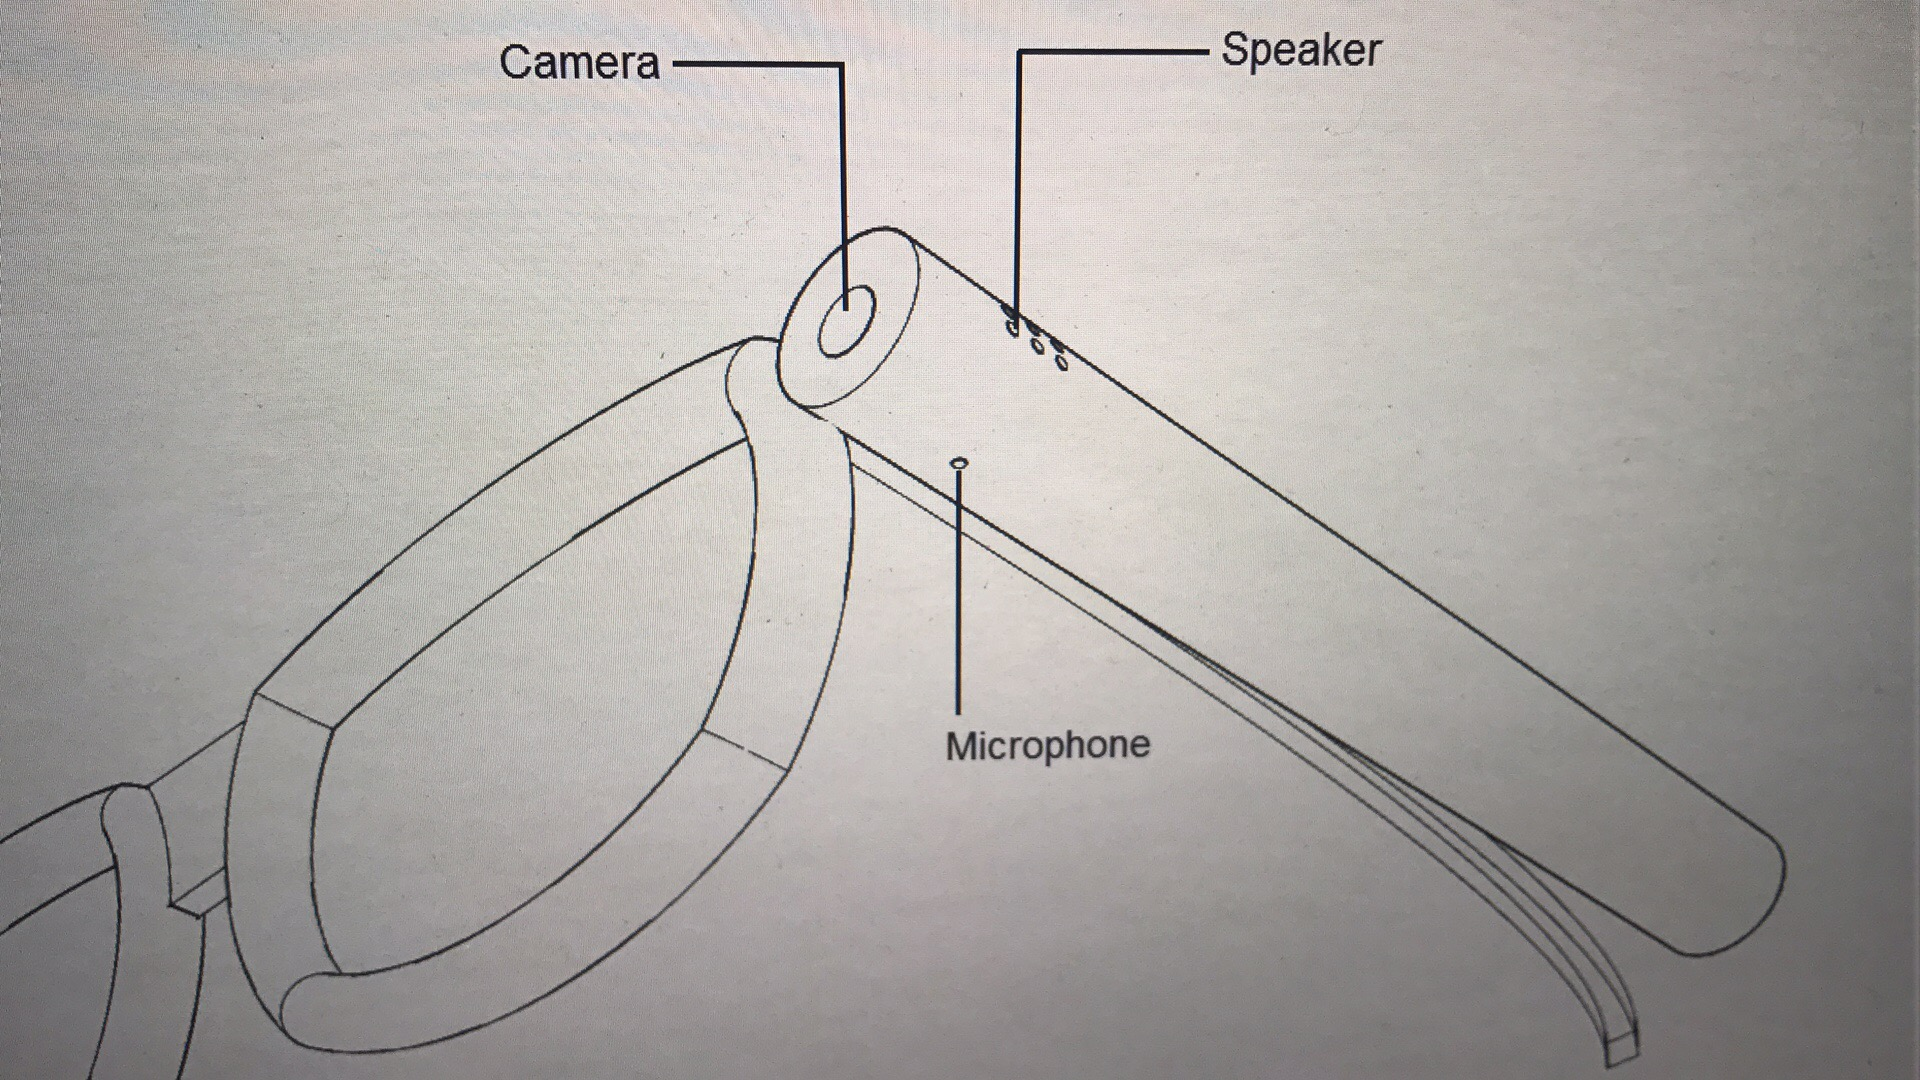
\includegraphics[width=\columnwidth]{device1}
\end{figure}

The physical properties of the SEDA had a cylinder shape, and a front camera used to capture what the driver was seeing, a speaker used to provide safe driving suggestion to the driver, a microphone used by the driver to trigger commands over voices, a Bluetooth component used to connect the device to the driver’s smartphone to provide extended user interfaces and to synchronize the driver’s driving data to the cloud intelligence service, a gyroscope to track the driver’s head movement, a lithium ion battery, a local memory to store temporary driving data and a low-power CPU for simple data processing. The device only comprised of simple components to make it light weight, has a long battery life and comfortable to wear. It recharged on docking station.

\begin{figure}
\caption{SEDA 3D design model}
\centering
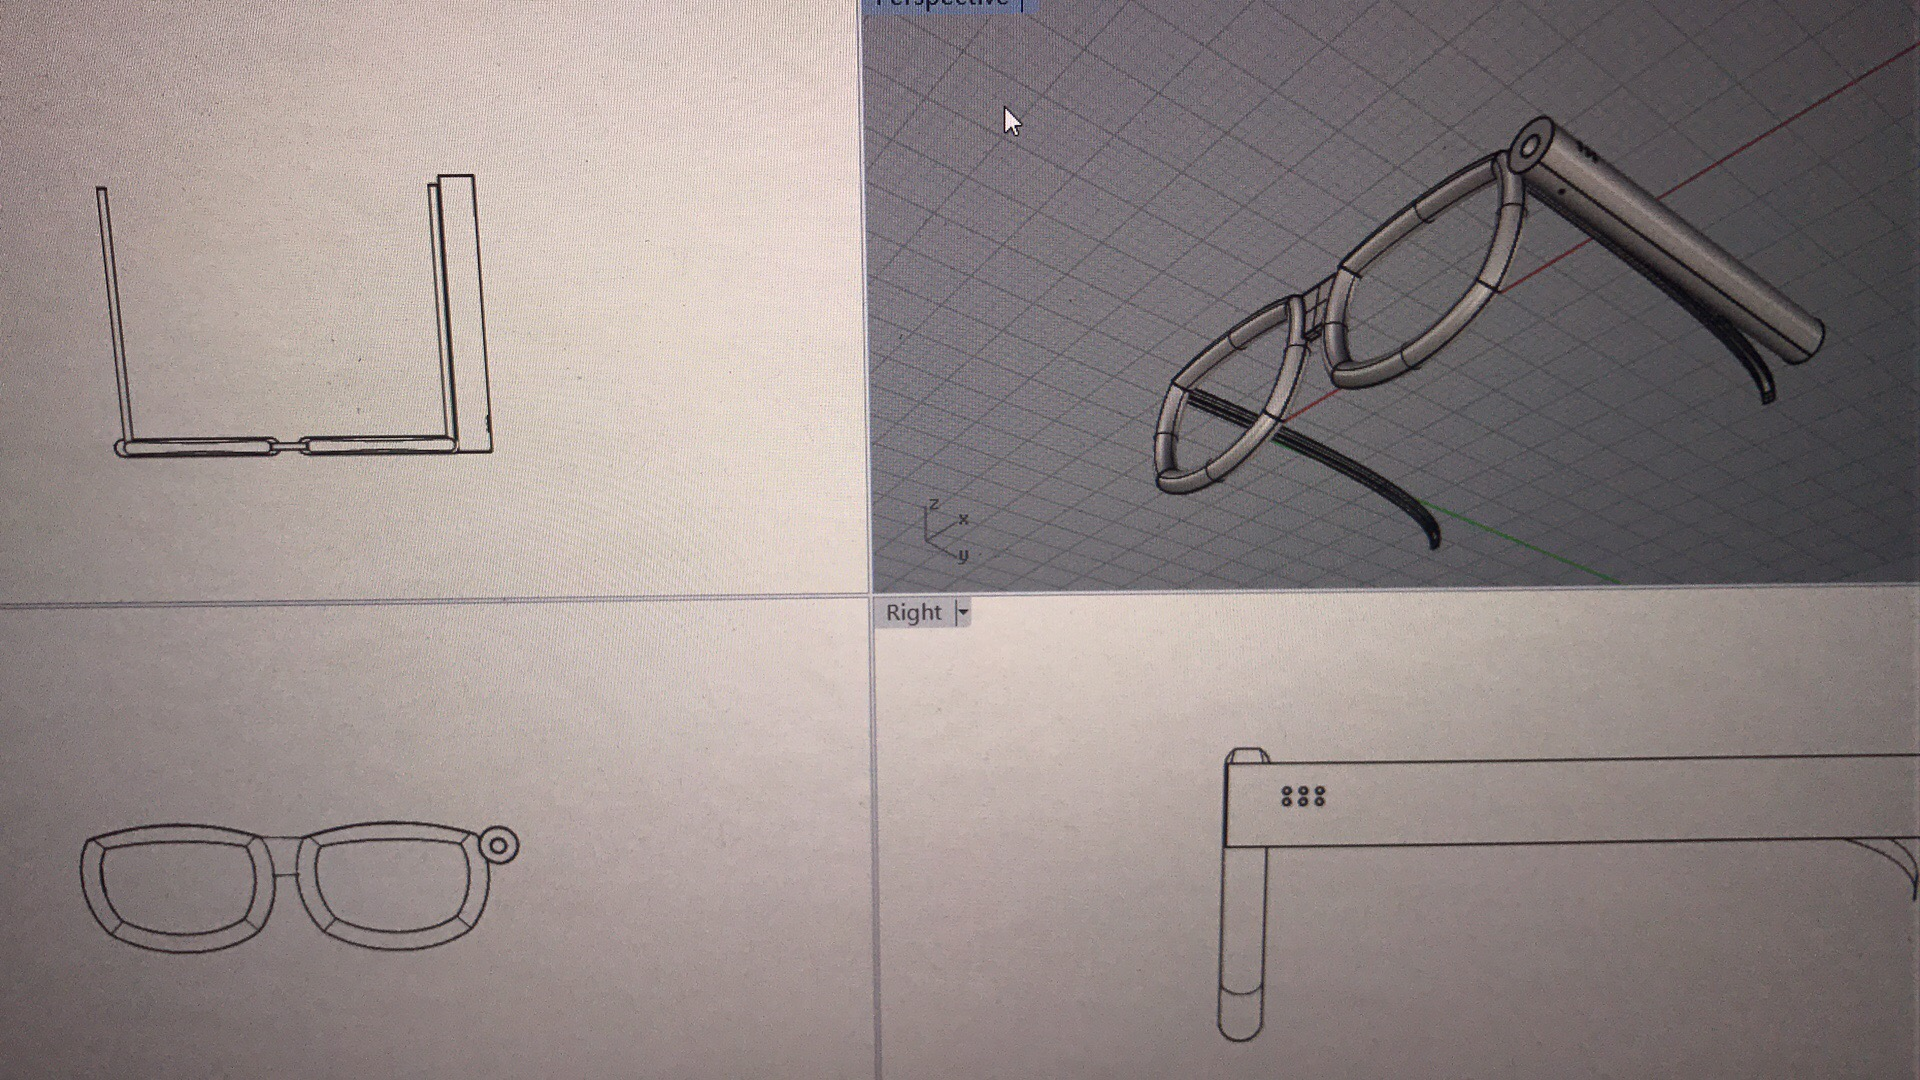
\includegraphics[width=\columnwidth]{device2}
\end{figure}

The SEDA was easily able to attach to the glasses with a magnet i.e. like Apple MacBook MagSafe connector. For the glasses made of non-magnetic material, we also provided a slip-pouch for the glass frame that would in place magnetically so that if it was tugged. It also designed to attach to head band if the driver had no wearing glasses. The camera was on the same level of the driver’s head. The camera was used to capture the surrounding images that were currently observed by the driver to make our system context-aware and combined with the gyroscope which was used to detect the head movement then our system had enough data to make an active advice on guiding the driver for safe driving \cite{murphy2010head, doshi2009roles}. 
\\
\\
\\
\\
\\
\\

\begin{figure}
\caption{SEDA attached to the glasses 2}
\centering
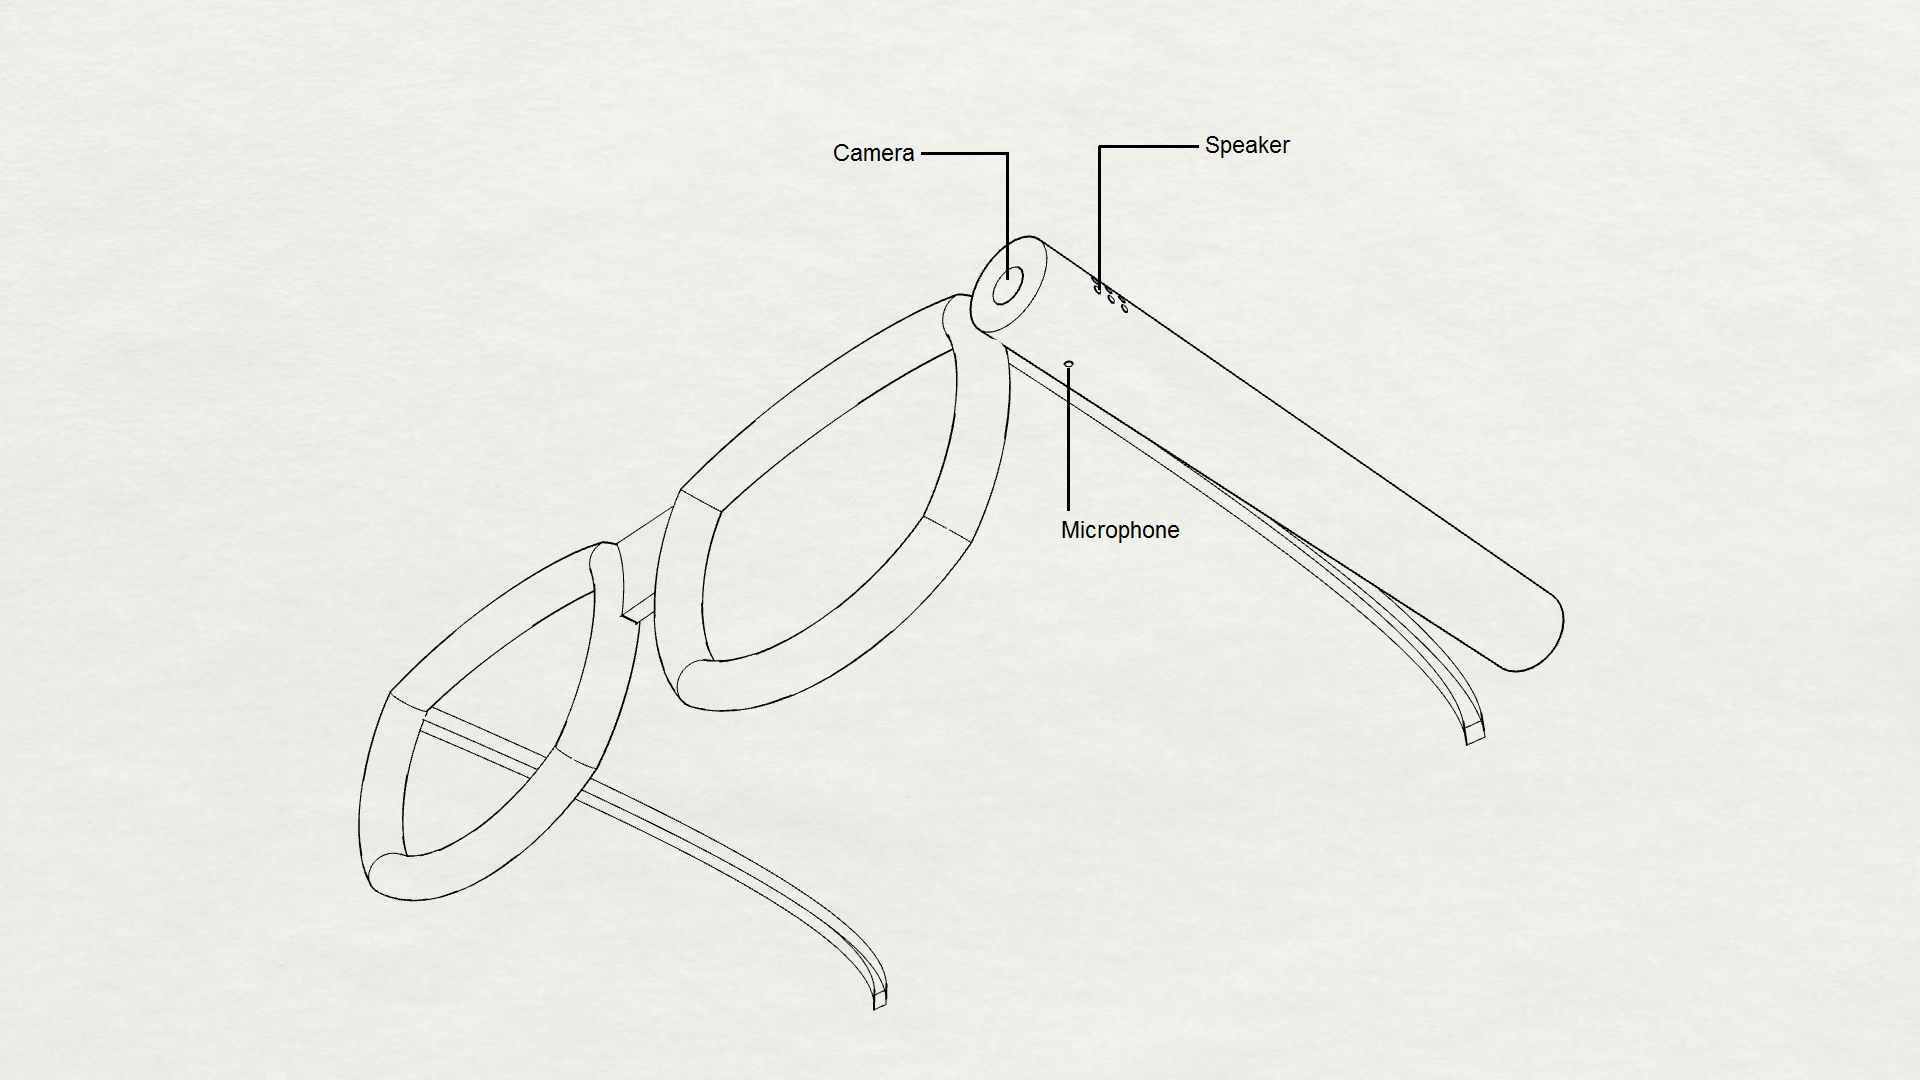
\includegraphics[width=\columnwidth]{device3}
\end{figure}

The speaker in our device was an essential output component for our system to train a safe driver. From the study \cite{rueda2004influence}, which explained the importance of passengers on the car could reduce the risk of causing the car collision, so our device was using the speaker to create a virtualize passenger (artificial intelligence) who was very good at helping the driver for safe driving.

\subsection{Discussion}

People might argue that the eye gaze could be a better choice than tracking of head movement, but the study of \cite{doshi2009roles} showed a strong evidence that detecting head movement was more accurate, easier and cheaper than using a second camera to track the driver’s eyes, since the tracking of gaze was affected by many factors like change of light intensity. Our device aimed to be light and has long battery life, so the second camera was not a good choice.

\end{document}